\documentclass[12pt]{article}

\usepackage{graphicx,amsmath,amsfonts,amssymb}
\usepackage{tikz}
\usepackage{cleveref}

\title{Vector Addition}

\author{Cameron Jordan}

\begin{document}
\maketitle

\section{Vector Representation}
What is a vector?, any mathematical object that has both magnitude and direction. Consider the number 5 on the real number line, here 5 is a vector that is five units from the origin in the positive direction, and is an example of a one dimensional vector. There are many ways by which we may represent vectors. Some of these ways are:

\begin{itemize}
\item $a\hat{i}+b\hat{j}+c\hat{k}$ where $a,b,c \in\mathbb{R}$ and $\hat{i},\hat{j},\hat{k}$ are the cardinal directions in 3-D, in 2-D $\hat{i},\hat{j}$ are commonly used. Beyond three dimensions it is common to use $\hat{x_1},\hat{x_2},\ldots,\hat{x_1}$ where each represents a cardinal direction in the space.
\item $\mathcal{h}x_1,x_2,\ldots,x_n\mathcal{i}$ where $x_1,x_2,\ldots,x_n\in\mathbb{R}$

\item $\begin{bmatrix}x_1\\x_2\\\vdots\\x_n\end{bmatrix}$ where $x_1,x_2,\ldots,x_n\in\mathbb{R}$

\item $\vec{x}$ to denote an arbitrary vector. Note $\vec{0}$ is commonly used to denote the vector with zero magnitude.

\item Graphically using an arrow in 2-D or 3-D, but not 4-D or higher because then it's hard to draw.
\end{itemize}

\section{How To}

We add vectors component-wise so given two $n$-dimensional vecors $\vec{x}=\mathcal{h}x_1,x_2,\ldots,x_n\mathcal{i}$ and $\vec{y}=\mathcal{h}y_1,y_2,\ldots,y_n\mathcal{i}$, \[\vec{x}+\vec{y}=\mathcal{h}x_1+y_1,x_2+y_2,\ldots,x_n+y_n\mathcal{i}\]

We can add vectors graphically via the \textbf{tail to tip} method. Note that two vectors that have the same magnitude and direction are equivalent no matter their position in the space.

\underline{The \textbf{tail to tip} method}

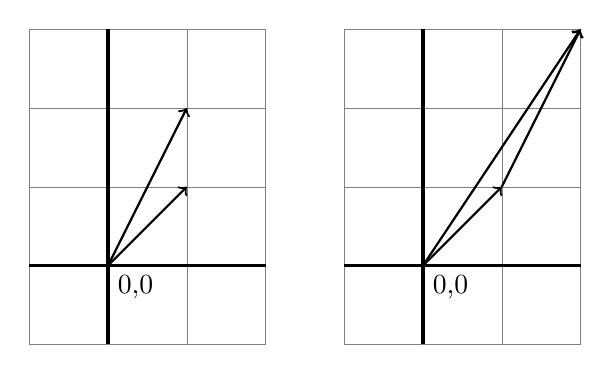
\begin{tikzpicture}
\draw[step=1cm, gray ,very thin] (-1,-1) grid (2,3);
\draw[very thick] (-1,0)--(2,0);
\draw[very thick] (0,-1)--(0,3);
\draw[->, thick] (0,0)--(1,1);
\draw[->, thick] (0,0)--(1,2);
\draw (0,0) node[anchor=north west] {0,0};

\draw[step=1cm, gray ,very thin] (3,-1) grid (6,3);
\draw[very thick] (3,0)--(6,0);
\draw[ very thick] (4,-1)--(4,3);
\draw[->, thick] (4,0)--(5,1);
\draw[->, thick] (5,1)--(6,3);
\draw[->, thick] (4,0)--(6,3);
\draw (4,0) node[anchor=north west] {0,0};
\end{tikzpicture}

\section{Activity: Space Domination}
Cut out the provided starships and torpedoes. Activity meant to be done in groups of 3.

\textbf{The rules:}

Play on the table top. 1 unit = 1 cm, adjust if needed. You can use rulers, meter sticks, tape measures or any other straight edge to represent vectors.

Each player's starship has 3 damage points. When a starship gets hit by a torpedo or another starship, it loses a damage point. If a starship reaches 0 damage points, flip it over and draw an `X' on the back. Should a starship's movement cause it to fly off the edge of the table the starship's damage points is reduced to 0.

Each player's starship starts with 3 torpedoes

Roll a six sided die to determine turn order, highest roll goes first. On your turn you can either move your starship or lauch a torpedo.

When your starship moves it accelerates in the direction it is pointing. Where your ship moves to is defined by a vector, $\vec{v}$, where:
\begin{equation}
\vec{v}=\vec{a}+\vec{r}\label{smoveq}
\end{equation}
calculated using the \textbf{tail to tip} method.

When your ship moves it produces an acceleration vector, $\vec{a}$, with magnitude in units equal to the value rolled on a six-sided die that is in the direction of your ship's acceleration. When the game begins $\vec{r}=\vec{0}$, so on your first move $\vec{v}=\vec{a}$. On your turn before you move $\vec{r}$ is set to the $\vec{v}$ of the previous turn. On your next move you can accelerate again producing a new vector, $\vec{v}$ via \cref{smoveq}.

While moving you may rotate your ship up to $180^\circ$ ($\pi$ radians) clockwise or counterclockwise.

When a torpedo is lauched the starship drifts along its $\vec{r}$. A topedo moves in the same fashion as a starship, but its initial direction is determined by the direction the launching starship is pointed, and the magnitude of the torpedo's $\vec{a}$ is always 6 units. A torpedo launched is not regained.\bigskip

\textbf{Win condition:} Be the last starship standing.\bigskip

\begin{tikzpicture}
\draw (0,0) node {\includegraphics[scale=2]{Space-Domination/StarshipGreen.png}};
\draw (2,0) node {\includegraphics[scale=2]{Space-Domination/StarshipRed.png}};
\draw (4,0) node {\includegraphics[scale=2]{Space-Domination/StarshipBlue.png}};
\draw (6,0) node {\textbf{Starships}};
\draw (6,-1.75) node {\textbf{Torpedoes}};
\draw (0,-1.5) node {\includegraphics[scale=1.5]{Space-Domination/torpedo.png}};
\draw (2,-1.5) node {\includegraphics[scale=1.5]{Space-Domination/torpedo.png}};
\draw (4,-1.5) node {\includegraphics[scale=1.5]{Space-Domination/torpedo.png}};
\draw (0.5,-2) node {\includegraphics[scale=1.5]{Space-Domination/torpedo.png}};
\draw (2.5,-2) node {\includegraphics[scale=1.5]{Space-Domination/torpedo.png}};
\draw (4.5,-2) node {\includegraphics[scale=1.5]{Space-Domination/torpedo.png}};
\draw (-0.5,-2) node {\includegraphics[scale=1.5]{Space-Domination/torpedo.png}};
\draw (1.5,-2) node {\includegraphics[scale=1.5]{Space-Domination/torpedo.png}};
\draw (3.5,-2) node {\includegraphics[scale=1.5]{Space-Domination/torpedo.png}};
\end{tikzpicture}\\\bigskip

Made using \LaTeXe
\end{document}